\section{Solver Convergence}
\subsubsection{NACA0012}
Figure \ref{fig:sc_NACA0012} shows the solver convergence for the NACA0012
testcase. The baseline implementation (marked as \textit{base}) and the final
state when writing this report (marked with \textit{modified}) is shown. Both
states were run once with 1 and 6 cpus.

\begin{figure}[H] \centering
    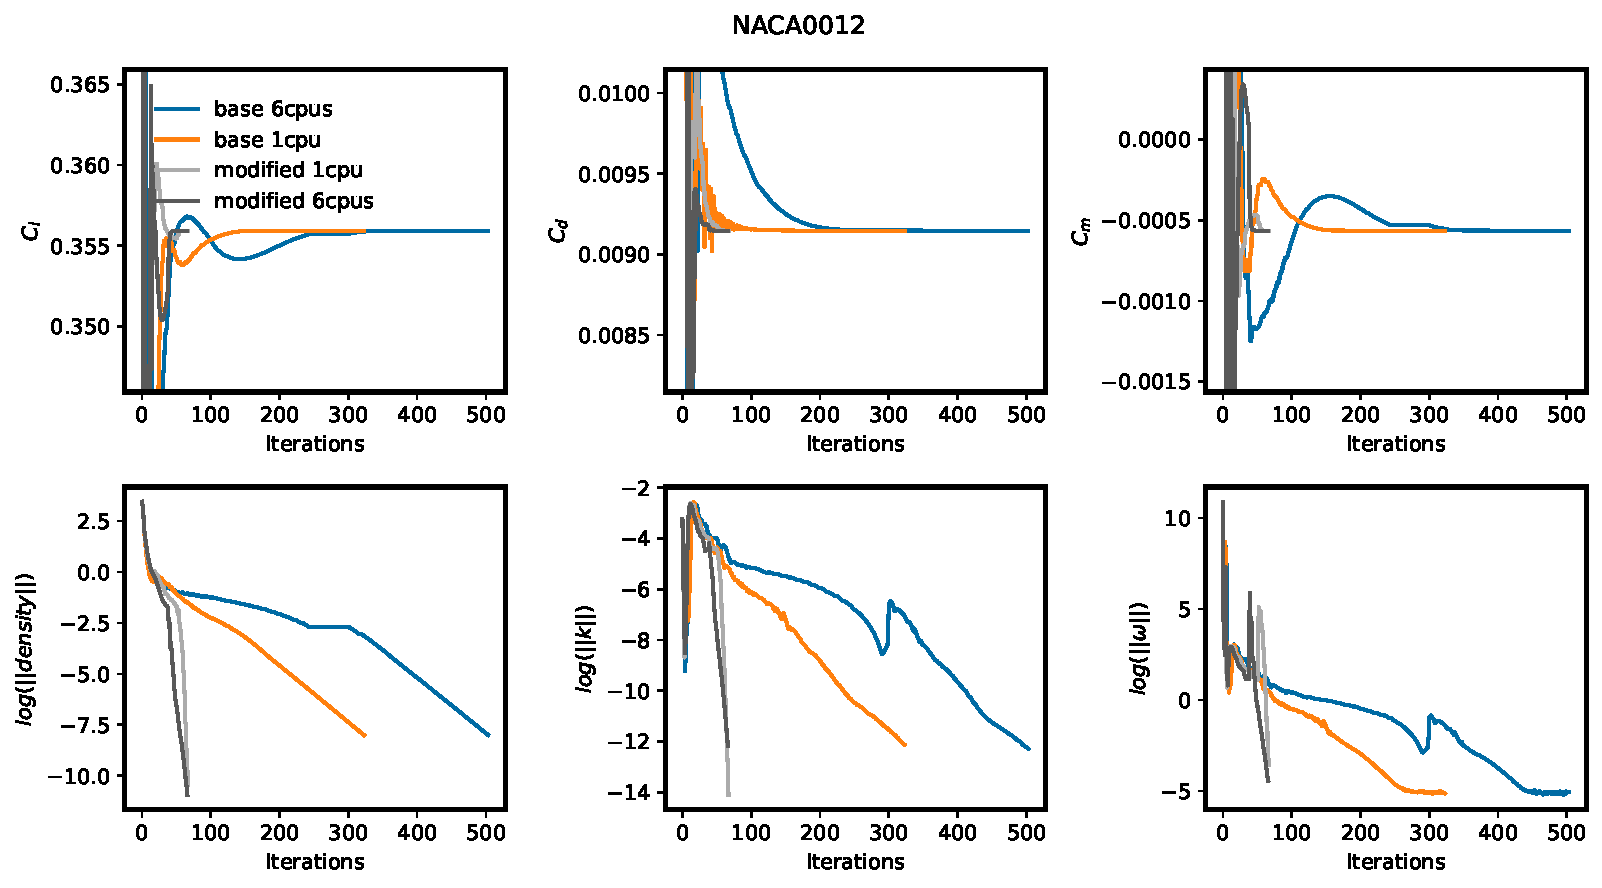
\includegraphics[width=1.0\textwidth]{plots/sc_NACA0012}
    \caption{Convergence history for NACA0012 testcase.}
    \label{fig:sc_NACA0012}
\end{figure}

\noindent Lets take a look at the baseline implementation first. It was
obtained using the ANK solver and a decoupled DADI solver for the turbulence
model. For the turbulence model, a total of 20 sub iterations were used. When
looking at the function values (top row), it can be seen that 1 and 6 cpus
reach the same value. But 6 cpus need more iterations. It is not quite clear
what causes this, but it is a known phenomenon for low cpu counts and vanishes
when this number is increased. Production runs usually require tens or even
hundrets of cpus and thus this is not considered detrimental.


Now, lets look at the modified implementation. Here, SST was differentiated and
the turbulence ANK and fully coupled CANK solvers are available. Annectdotal
evidence suggest SST is highly non-linear. This is especially true for the
inital stages of convergence. Due to this\footnote{The author believes the ANK
solver does some finite-differencing for some terms under the hood.}, the
turbulence DADI solver is way more efficient early on. Thus, at the beginning,
the regular ANK solver with decoupled DADI was used. But once a relative
convergence of 1e-6 is reached, the second order coupled ANK (CSANK) is
engaged. Once it gets traction, it exhibits almost Newton-like convergence. The
number of cpus does not really affect the number of iterations needed. It is
also obvious that the modified version approaches the same function values as
the baseline implementation. 




\subsubsection{RAE2822}
Figure \ref{fig:sc_RAE2822} shows a similar convergence plot for the RAE2822
testcase. Once again, the baseline and modified version with each 1 and 6 cpus
is plotted. It is important to note that this case is somewhat hard as it lies
in the transsonic regimes where shocks appear. But at the same time, it is even
coarser than the NACA case which makes it hard to resolve the shocks properly.

\begin{figure}[H] \centering
    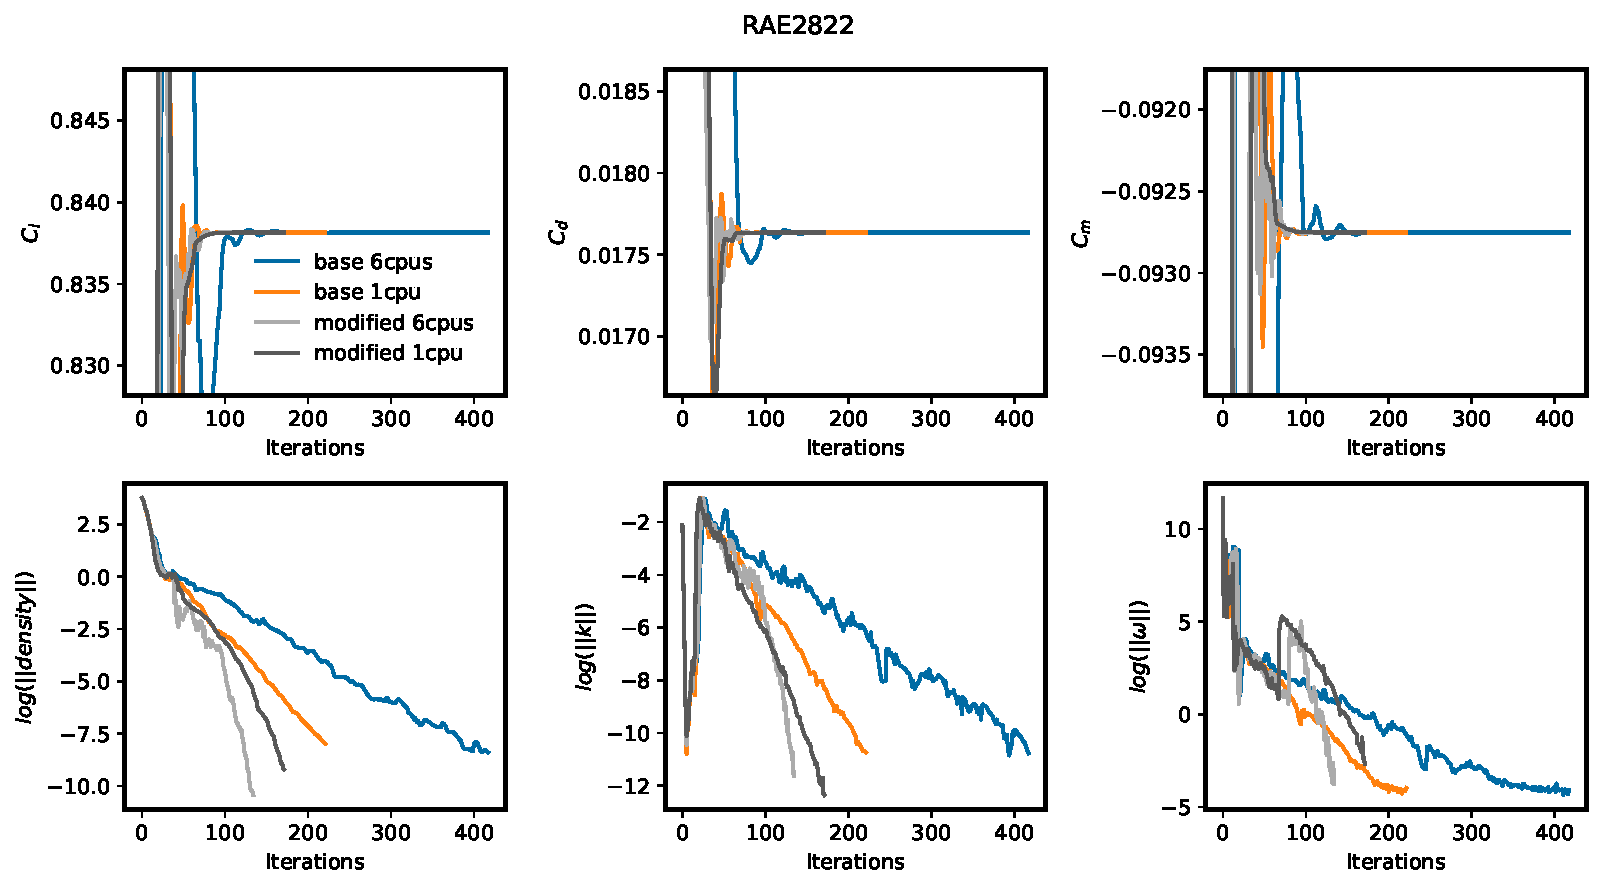
\includegraphics[width=1.0\textwidth]{plots/sc_RAE2822}
    \caption{Convergence history for RAE2822 testcase.}
    \label{fig:sc_RAE2822}
\end{figure}

\noindent First, lets glance at the baseline. This has also been obtained
using the ANK solver for the flow variables and the DADI solver for the
decoupled turbulence variables. A similar pattern to the NACA
testcase appears: 1 cpu takes only half the iterations of what 6 cpus need.
But, the converged values are the same. 

When looking at the general line pattern and comparing it to the NACA testcase,
it appears to be more 'wiggly'. The author believes this is due to SST being
highly non-linear which is exaggerated by the appearances of transsonic shocks.
This leads to a high sensitivity to the CFL number. The ANK solver uses a
CFL-ramping algorithm that increases the CFL number steadily the closer to
convergence it is. This ramping algorithm is not dumb and uses a smart
formulation that also reduces the CFL number when the ANK solver has problems
solving the linear system for the current step. The author believes herein lies
the problem: the high non-linearity of SST and the fact that this
ramping-algorithm is tuned for SA. This leads to a coupling where the ANK
solver would increase the CFL number to much and start diverging. Once this is
detected, the CFL number is lowered once again an convergence continues. 

When looking at the modified version, a similar picture to NACA emerges. The
strategy was the same, first use ANK with DADI and once a relative convergence
of 1e-6 is reached, the CSANK solver is enganged which shows almost Newton-type
convergence. Although the contrast is not as big. But it also has to be noted
that that the before mentioned CFL dependence played a role here and some
parameters had to be clipped to increase robustness at the cost of convergence.





\section{Grid Convergence}
Figure \ref{fig:gc_2d_bump} shows the grid convergence for the 2d bump testcase
compared to data from the \textit{CFL3D} and \textit{FUN3D} CFD solvers. At
first glace, ADflow seems to be in the right bulk part but does not completely
agree with the reference. This difference may be explained through slightly
different model formulations and production terms. Usually, a formulation know
as \textit{vorticity} is used. The author tried to converge this testcase using
it but was unable to do so. So the results shown where obtained using the
\textit{strain} turbulence production formulation. It is also not completely
clear what version of SST was implemented in ADflow which might skew the
results even more. The reference data was obtained using the \textit{SSTm}
formulation. 

\begin{figure}[H] \centering
    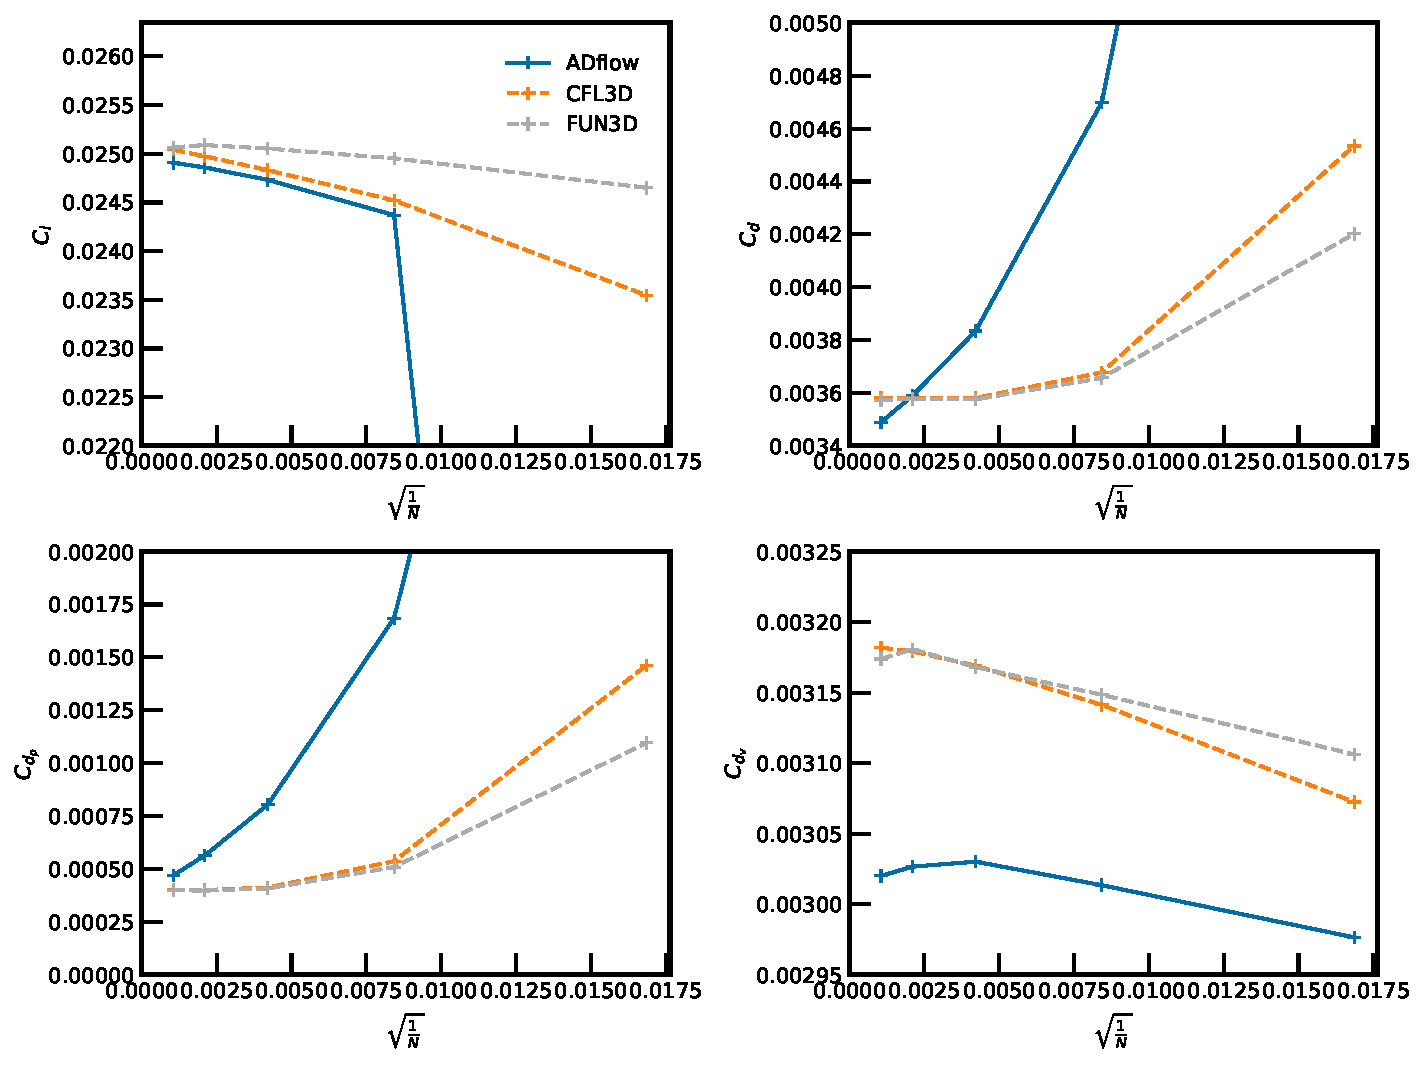
\includegraphics[width=1.0\textwidth]{plots/gc_2d_bump_nan-fix}
    \caption{Grid convergence for 2D bump. Reference data is from
    \cite{nasatmr}.}
    \label{fig:gc_2d_bump}
\end{figure}

\noindent But ignoring the discrepancies, one can observe that the values
appear to smoothly approach a limit.







\section{Partial derivatives}
\subsubsection{Forward mode}
To verify the forward partial derivatives, the 3D test case is first converged
to a relative tolerance of $1e-14$.\footnote{In theory, the partials should be
accurate regardless of the current convergence. But it is more valuable when
one can show that they are accurate for a converged state as this is what we
are after. } Once this is the case, the partials are compared against finite
difference and complex step. Anecdotal evidence suggest SST is highly
non-linear which is reflected in the fact that the FD partials are quite off
compared to AD (The maximum observed difference was in the order of $1e2$).
Table \ref{tab:partials_forward} lists the derivatives with the relative
accuracy compared to CS (stepsize was $1e-40$). 
\begin{table}[H]
    \centering
    \begin{tabular}{l r}
        \toprule
        Derivative                          & Relative tolerance \\
        \toprule
        $\partial R / \partial u$           & $\leq 1e-9$ \\
        $\partial f / \partial u$           & $\leq 1e-9$ \\
        $\partial F / \partial u$           & $\leq 1e-9$ \\
        \midrule
        $\partial R / \partial x_{geo}$     & $\leq 1e-9$ \\
        $\partial f / \partial x_{geo}$     & $\leq 1e-9$ \\
        $\partial F / \partial x_{geo}$     & $\leq 1e-9$ \\
        \midrule
        $\partial R / \partial x_{aero}$    & $\leq 1e-10$ \\
        $\partial f / \partial x_{aero}$    & $\leq 1e-10$ \\
        $\partial F / \partial x_{aero}$    & $\leq 1e-10$ \\
        \bottomrule
    \end{tabular}
    \caption{Relative accuracy of forward AD partials compared to CS.}
    \label{tab:partials_forward}
\end{table}

\noindent This exact testcase is used in regression test that make sure new
features do not break existing ones. Usually a tolerance of $1e-10$ is need to
pass this test. But due to the non-linearity of SST, this had to be lifted to
$1e-9$. Of course, this is only lifted for SST and the other turbulence models
still need to pass $1e-10$.


\subsubsection{Reverse mode}
To verify the backwards partials, a dot-product test was performed. It is also
part of the regression test-suite. Table \ref{tab:partials_dotproduct_test}
lists each test with the relative tolerance it achieved. The only test that
did not pass was $u \rightarrow F$. As $F$ are the nodal forces, those
derivatives are only needed for aerostructural optimization. The reason for
failing is probably the fact, that those routines buffer some values without
recomputing. The changes to the wall distance probably require changes to those
buffered routines as well. As this was not done, the test fails.

\begin{table}[H]
    \centering
    \begin{tabular}{l r}
        \toprule
        Dot product test                     & Relative tolerance \\
        \toprule
        $u \rightarrow R$                   & $\leq 1e-10$ \\
        $u \rightarrow F$                   & $\textcolor{red}{= 2e-6}$ \\
        \midrule
        $x_{geo} \rightarrow R$             & $\leq 1e-9$ \\
        $x_{geo} \rightarrow F$             & $\leq 1e-10$ \\
        \midrule
        $(u, x_{geo}) \rightarrow (du, F)$  & $\leq 1e-10$ \\
        \bottomrule
    \end{tabular}
    \caption{Relative accuracy of dot product test between forwards and
    backwards partial derivatives.}
    \label{tab:partials_dotproduct_test}
\end{table}


\subsubsection{Reverse\_fast mode}
The regression test for the reverse\_fast partials simply compares them to the
forwards routines. This is possible because the fast routines are a subset of
the normal ones. Table \ref{tab:partials_fast} lists the relative accuracy. It
obviously does not agree at all. Unfortunately, the author did not have enough
time to properly debug this. But the fact that it yields a number and does not
simply crash is already an achievement.

\begin{table}[H]
    \centering
    \begin{tabular}{l r}
        \toprule
        backwards vs backwards\_fast        & Relative tolerance \\
        \toprule
        $u$                                 & $\textcolor{red}{= 5.7e4}$ \\
        \bottomrule
    \end{tabular}
    \caption{Relative accuracy of backwards\_fast routines compared to
    backwards.}
    \label{tab:partials_fast}
\end{table}







\section{Total derivatives}
As described in sec. XXX, the total derivatives were verified by comparing them
to complex step. As described in sec. XXX, ADflow may assemble the adjoint
system using either the forwards partials or the reverse\_fast partials. Table
\ref{tab:total_derivs} lists the relative difference of various methods
compared against complex step with a stepsize of $1e-200$.

\begin{table}[H]
    \centering
    \begin{tabular}{l r r r r}
        \toprule
        Name        & cmplx. ($h=1e-40$)   & adj. frwd. 1cpu           & 
            adj. frwd. 6 cpus         & adj. rev. fast 6 cpus    \\
        \toprule
        alpha       & -1.3e-09             & -5.3e-06                  & 
            -5.3e-06                  & \textcolor{red}{-8.0e-03} \\
        mach        & -6.1e-08             &  2.3e-05                  &  
            2.3e-05                  & \textcolor{red}{ 2.3e-01} \\
        \midrule
        span \#0    & -2.0e-09             &\textcolor{red}{ 4.0e-04}  &
            \textcolor{red}{-9.0e-04}  & \textcolor{red}{-1.0e-02} \\        
        twist \#0   &  9.3e-09             &\textcolor{red}{-1.0e-03}  &
            9.6e-05                    & \textcolor{red}{-1.4e-02} \\        
        shape \#0   & -5.3e-07             &\textcolor{red}{ 5.8e-02}  &
            \textcolor{red}{ 5.6e-02}  & \textcolor{red}{ 1.2e-00} \\         
        \bottomrule
    \end{tabular}
    \caption{Relative difference of gradients compared to compplex step
    (stepsize = 1e-200). The function of interest is $C_l$. When the DVs are a
    vector (e.g span), only the first variable is listed.}
    \label{tab:total_derivs}
\end{table}

\noindent First, lets look at the forward routines with 1 and 6 cpus. The first
two variables are \textit{aerodynamic}, which means that they do not control
the geometry. It appears that they stay the same on 1 or 6 cpus. Their relative
accuracy is approx 1e-5. This is relatively low, but may be explained through
the high non-linearity of SST. It is also important to realize that this is
the first guesses into the blue regarding options and tuning. One can probably
expect a higher accuracy once more time is spend on the problem and the correct
options are found.

When looking at the \textit{geometric} derivatives (such as span, twist and
shape), it becomes clear that they depend on the number of cpus. Also, they are
less accurate than the geometric ones. This probably indicates a problem with
the modification done to the wall distance exchange routines. Due to time
constraints, it was not possible to fix it.

As already indicated with the partial reverse\_fast routines, the total
derivatives are also completely wrong. But once again, the fact that a number
was obtainable is already an achievement. It is expected that this will be
fixed once more time is spent on the problem.







\section{Summary}
The results show that a prototype state was achived. SST does converge using
the coupled ANK solver and also gradients can be obtained. But of course, there
are still some bugs present. Some other results were more anecdotal and could
not be proven scientifically in this project. The following list summarizes the
insights (anecdotal and proven) gained through the course of this project.

\begin{itemize}
    \item SST is probably highly non-linear.

    \item ANK does work using the AD preconditioner. But sometimes NaNs appear.

    \item ANK does not work using FD preconditioner (probably due high
        non-lineary of SST).

    \item Physicality check for ANK needs to be adjusted to SST.

    \item Prototype adjoint is running.

    \item Aerodynamic derivatives using forward routines are accurate.

    \item Geometric derivatives using forward routines are not accurate.

    \item There is probably a bug in the halo exchange of the wall distance in
        the backwards routines.

    \item Derivatives using reverse\_fast routines are not accurate at all.

    \item SST appears to be implemented correctly.
\end{itemize}
